Create a new Class and name it "World". Edit the buffer so it looks as follows and then save it:\\\\
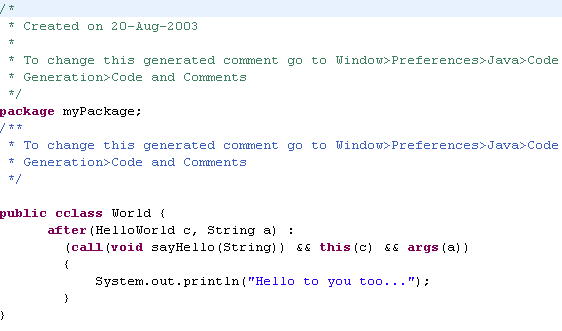
\includegraphics[width=0.80\textwidth]{images/aspect.png}\\

Make a clean Build of the project, and the outline view populates. Expand the "after()" node.\\\\
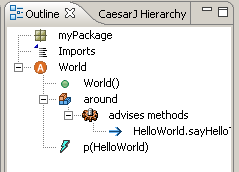
\includegraphics[width=0.5\textwidth]{images/aspect2.png}\newpage

You can see that this advice is affecting the HelloWorld.sayHello() method. Clicking on the "HelloWorld.sayHello()" node in the outline takes you to the declaration of HelloWorld.sayHello().

Notice the "advice annotation" in the editor buffer (highlighted) and that the "sayHello" method in the outline view shows that it is advised by the World aspect.\\\\
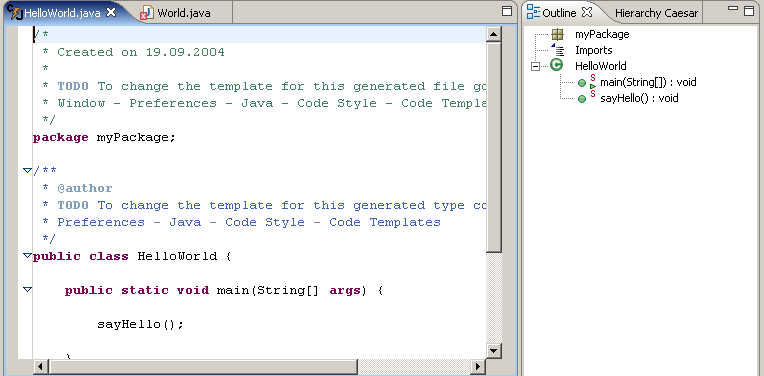
\includegraphics[width=0.95\textwidth]{images/aspect3.png}\\\\

Selecting the "World.after()" node in the outline view takes you back to the advice declaration. Right-clicking on the advice annotation brings up a context menu that also allows you to navigate to the advice.\\\\
\textbf{TODO BILD FEHLT KONNTE ICH NICHT SCREENSHOOT MACHEN  Weil es nicht geht EDITOR mit ADVICE CONTEXT}

